\documentclass[xcolor=dvipsnames]{beamer}
\usetheme{nelle}
\usepackage{natbib}                 % Fancy bibliography.
\usepackage{url}                    % Allow printing of URLs.
\usepackage{outlines}
\usepackage{enumitem}
\usepackage{multicol}
\usepackage{dsfont}
\usepackage{amsmath}
\usepackage{epstopdf}
\usepackage{listings}
\usepackage{color}
\setbeamerfont{caption}{size=\scriptsize}
\setbeamertemplate{navigation symbols}{}
\setbeamertemplate{footline}[frame number]{}

\def\newblock{\hskip .11em plus .33em minus .07em}
\usepackage{color}

\definecolor{mygreen}{rgb}{0,0.6,0}
\definecolor{mygray}{rgb}{0.5,0.5,0.5}
\definecolor{mymauve}{rgb}{0.58,0,0.82}

\lstset{ %
  backgroundcolor=\color{white},   % choose the background color; you must add \usepackage{color} or \usepackage{xcolor}; should come as last argument
  basicstyle=\scriptsize,        % the size of the fonts that are used for the code
  breakatwhitespace=false,         % sets if automatic breaks should only happen at whitespace
  breaklines=true,                 % sets automatic line breaking
  captionpos=b,                    % sets the caption-position to bottom
  commentstyle=\color{mygreen},    % comment style
  deletekeywords={...},            % if you want to delete keywords from the given language
  escapeinside={\%*}{*)},          % if you want to add LaTeX within your code
  extendedchars=true,              % lets you use non-ASCII characters; for 8-bits encodings only, does not work with UTF-8
  keepspaces=true,                 % keeps spaces in text, useful for keeping indentation of code (possibly needs columns=flexible)
  keywordstyle=\color{blue},       % keyword style
  language=Python,                 % the language of the code
  morekeywords={*,...},            % if you want to add more keywords to the set
  rulecolor=\color{black},         % if not set, the frame-color may be changed on line-breaks within not-black text (e.g. comments (green here))
  showspaces=false,                % show spaces everywhere adding particular underscores; it overrides 'showstringspaces'
  showstringspaces=false,          % underline spaces within strings only
  showtabs=false,                  % show tabs within strings adding particular underscores
  stringstyle=\color{mymauve},     % string literal style
  tabsize=2,                     % sets default tabsize to 2 spaces
  title=\lstname                   % show the filename of files included with \lstinputlisting; also try caption instead of title
}

\newcommand{\todo}[1]{\textbf{[TODO: #1]}}
\newcommand{\fixme}[1]{\textbf{[FIXME: #1]}}


\title{\textbf{The Scientific Python Toolstack for biomedical research}}

\author[Varoquaux Nelle]{
Nelle Varoquaux}


\date{December, 3rd}
\institute{Mines ParisTech, Institut Curie, INSERM}
\begin{document}
\begin{frame}[t, noframenumbering]
  \maketitle

\end{frame}

\setcounter{framenumber}{0}

\begin{frame}
\frametitle{The DNA sequence holds the genetic information}
\begin{columns}
\begin{column}{0.45\linewidth}
\includegraphics[width=\linewidth]{images/bio_101.png}
\end{column}
\begin{column}{0.45\linewidth}
\begin{itemize}[label={$\bullet$}]
\item Beings are composed on one or several cells.
\item Cells contain the genetic code of an individual on the DNA sequence.
\item This DNA sequence is roughly identical between organisms, and between cell of an organism.
\end{itemize}
\end{column}
\end{columns}
\end{frame}

\begin{frame}
\frametitle{Several genome sizes}

\begin{table}
\footnotesize
\begin{tabular}{l | l | l | c}
{\bf Organisms} &{\bf Chromosomes} & {\bf Size} & {\bf Ratio} \\
\hline
{\bf Bacteria} & 1 & 400,000 to 10,000,000 & $\leq 1$ \\
{\color{Blue} \bf In search of lost time} & 7 & 9,609,000 & 1\\
{\bf Yeast} & 12 & 14,000,000 & 1.5 \\
{\bf Fly} & 4 & 300,000,000 & 30 \\
{\bf Human} & 46 & 6,000,000,000 & 600 \\
{\bf Tulip} & 60 & 30,000,000,000 & 3,000 \\
\end{tabular}
\end{table}
\end{frame}

\begin{frame}
\frametitle{As sequencing costs diminish\dots}
\begin{figure}
\includegraphics[width=0.9\linewidth]{images/dna_sequences_growth.PNG}
\end{figure}
\end{frame}


\begin{frame}
\frametitle{How can we analyse such large quantity of data?}
\begin{figure}
\includegraphics[width=0.9\linewidth]{images/dna_sequences_growth.PNG}
\end{figure}
\end{frame}

\begin{frame}
\frametitle{Can we use the Scientific Python Toolstack?}

\begin{center}
\includegraphics[width=0.2\linewidth]{images/pythonlogo.jpg} \hspace{3em}
\includegraphics[width=0.2\linewidth]{images/numpy.jpg}\hspace{3em}
\includegraphics[width=0.2\linewidth]{images/scipy.jpg}
\end{center}

\vspace{1.5em}

\begin{center}
\hspace{3em}
\includegraphics[width=0.2\linewidth]{images/scikit-learn.png}\hspace{3em}
\includegraphics[width=0.2\linewidth]{images/ipython.jpg}\hspace{3em}
\includegraphics[width=0.2\linewidth]{images/matplotlib.png}
\end{center}
\end{frame}

\begin{frame}
\frametitle{}
{\Large \bf A couple of examples of projects accomplished in Python}
\end{frame}

\begin{frame}
\frametitle{``Cell cognition''}
\begin{center}
\includegraphics[width=0.6\linewidth]{images/cell_cognition.png}
\end{center}
\end{frame}

\begin{frame}
\frametitle{DREAM challenge: predicting the toxicity of drugs}
\begin{center}
\includegraphics[width=0.7\linewidth]{images/toxicogenetic_challenge.png}
\end{center}
\end{frame}

\begin{frame}
\frametitle{What are you thinking of?}
\begin{center}
\includegraphics[width=0.5\linewidth]{images/brain_activity.png}
\end{center}
\end{frame}


\begin{frame}
\frametitle{My personal interest: the 3D structure of the genome}
\begin{columns}
\begin{column}{0.45\linewidth}
\includegraphics[width=\linewidth]{images/bio_101.png}
\end{column}
\begin{column}{0.45\linewidth}
\begin{itemize}[label={$\bullet$}]
\item On the average, a single human chromosome consists of DNA molecule that is about 5cm long
\item A nucleus is on average 6$\mu$m of diameter.
\item {\bf \color{Blue} How does DNA fit into the nucleus?}
\end{itemize}
\end{column}
\end{columns}
\end{frame}

\begin{frame}
\frametitle{The 3D structure of the genome is thought to play an important
role in many biological processes}
\vspace{-0.6em}
\begin{figure}
\begin{center}
\includegraphics[width=0.7\linewidth]{figures/yeasts_genome_architecture.jpg}
\end{center}
\caption{\textbf{The genome of \textit{S. cerevisiae} is highly organized}
         \citep{zimmer:principles}}
\end{figure}
\end{frame}

% 2. What is the Hi-C protocol?
\begin{frame}
\frametitle{The Hi-C protocol identifies physical contacts between
pairs of loci genome-wide}
\begin{figure}
\centering
\includegraphics[width=0.85\textwidth]{figures/hic_protocol.jpg}
\caption{\textbf{Hi-C paves the way for a systematic and genome-wide analysis
of genome architecture} \citep{rao:3d}}
\end{figure}
\end{frame}

% 3. A contact count matrix
\begin{frame}
\frametitle{The contact count matrix recapitulates the hallmarks of genome
architecture}
\vspace{-1em}
\begin{figure}
\includegraphics[width=0.55\textwidth]{figures/yeast_counts.pdf}
\caption{\textbf{Contact counts for the first 5 chromosomes of \textit{S.
cerevisiae}}}
\end{figure}
\end{frame}

\begin{frame}
\frametitle{The computational challenges of Hi-C data}
\begin{itemize}[label={$\bullet$}]
\item The size of the organisms studied is growing.
\item The resolution is getting higher.
\item A 1~kb human map is 3,000,000 by 3,000,000.
\item In a naive format, {\bf this corresponds to 1.1~Tb of data}
\end{itemize}
\end{frame}


\section{ICE: how good data structure beats parallelization}
\begin{frame}
\Large{ \bf
\texttt{Iced}: Normalization of Hi-C data}

\begin{flushright}
\vspace{1em}
\small
\textit{How appropriate use of data structures beats C++ parallized code.}
\end{flushright}
\end{frame}

\begin{frame}
\frametitle{Contact-maps normalization: the ICE method}

{\bf \color{Blue} Sequencing data is full of biases}

\begin{itemize}[label={$\bullet$}]
\item Sequencing biases
\begin{itemize}
\item ("CG" riched regions are sequenced less than "AT" rich region)
\end{itemize}
\item The protocol induces more biases.
\end{itemize}
\vspace{3em}

\begin{center}
{\bf \color{Blue} We need to correct for these biases}
\end{center}

\end{frame}


\begin{frame}
\frametitle{Iterative Correction of Contact maps}
{\bf \color{Blue} Two hypotheses}

Denote by $C$ the raw contact count matrix and by $N$ the normalized one.

\begin{itemize}[label={$\bullet$}]
\item Each row and column interacts as much as any over row and column.
$$
\sum_{i} N_{ij} = K
$$
\item The bias of each entry of the matrix can be decomposed as the product of
a row and column-specific bias
$$
\beta_{ij} = \beta_i \beta_j
$$
\end{itemize}
\end{frame}

\begin{frame}
\frametitle{Formulating an optimization problem}
\begin{equation*}
\renewcommand{\arraystretch}{2}
\begin{array}{ccll}
\text{Find} & & \beta \\
\text{Such that} & & \underset{i}{\sum} \quad \beta_i \beta_j c_{ij} = K
\end{array}
\end{equation*}

\vspace{1em}
{\bf \color{Blue} Matrix-balancing problems} \\
\begin{itemize}[label={$\bullet$}]
\item This boils down to solving a {\bf matrix-balancing} problem.
\item These belong to an extremely widely studied class of problems.
\end{itemize}
\end{frame}

\begin{frame}
\frametitle{The Sinkhorn-Knopp algorithm}
{\bf \color{Blue} A very simple algorithm exists to solve this issue.}
\lstinputlisting{scripts/algorithm}
\end{frame}

\begin{frame}
\frametitle{A simple implementation}
\lstinputlisting{scripts/ice.py}
\end{frame}

\begin{frame}
\frametitle{A problem with the simple implementation}
\begin{center}
\begin{centering}
{\bf \color{Red} \Large This will not scale!}
\end{centering}
\end{center}
\end{frame}

\begin{frame}
\frametitle{Using scipy.sparse matrices !}
{\bf \color{Blue} Property of our data}
\begin{itemize}[label={$\bullet$}]
\item Our data is sparse (most of it is 0):
\item Our data is a symmetric matrix;
\item \texttt{scipy.sparse} can store sparse matrix and provide ``numpy-like'' interface.
\end{itemize}

\begin{columns}
\begin{column}{0.5\linewidth}
\end{column}
\begin{column}{0.5\linewidth}
\lstinputlisting{scripts/coo_data}
\end{column}
\end{columns}
\end{frame}

\begin{frame}
\frametitle{Using Sparse Compressed Row format}
{\bf \color{Blue} The CSR format}

\begin{itemize}[label={$\bullet$}]
\item \texttt{indices} is array of column indices
\item \texttt{data} is array of corresponding nonzero values
\item \texttt{indptr} points to row starts in indices and data
\item length is \texttt{n\_row + 1}, last item = number of values = length of both indices and data
\item nonzero values of the i-th row are \texttt{data[indptr[i]:indptr[i+1]]} with column indices \texttt{indices[indptr[i]:indptr[i+1]]}
\item item $(i, j)$ can be accessed as \texttt{data[indptr[i]+k]}, where $k$ is position of $j$ in \texttt{indices[indptr[i]:indptr[i+1]]}
\end{itemize}
\end{frame}


\begin{frame}
\frametitle{In short\dots}
{\Large \bf \color{Blue} It's roughly the same as COO for sums over row.}\\
\vspace{1em}
{\Large \bf \color{Blue} But sometimes we need to loop over
elements to perform operations}\\
\vspace{1em}
{\Large \bf \color{Blue} \flushleft And looping is slow\dots}
\end{frame}

\begin{frame}
\frametitle{Cython to the rescue}
\only<1>{
\begin{center}
\includegraphics[width=0.5\linewidth]{images/cython.png}
\end{center}
}
\only<2>{

\lstinputlisting{scripts/cython_normalization.pyx}
}
\end{frame}


\begin{frame}
\frametitle{How does our Cython/Python implementation perform?}

{HiCorrector is a C++ implementation of the same algorithm, parallelized but using dense format.}

\vspace{2em}
\begin{table}
\scriptsize
\begin{tabular}{l | c | c | c | c }
  & {\bf Iced {\tiny (dense)}} & {\bf Iced {\tiny (sparse)}} & {\bf HiCorrector {\tiny (1 CPU)}} & {\bf HiCorrector {\tiny (8 CPUs)}} \\
\hline
IMR90 1~Mbp & 00:00:12 & 00:00:25 & 00:00:25 & 00:00:06 \\
IMR90 500~kbp & 00:00:40 & 00:01:30 & 00:02:15 & 00:00:22 \\
IMR90 150~kbp & - & 00:04:28 & 00:13:21 & 00:03:10 \\
IMR90 40~kbp & - & 00:07:19 & 02:35:34 & 00:35:43 \\
IMR90 20~kbp & - & 00:08:36 & 12:57:17 & 02:34:05 \\
\end{tabular}
\end{table}
\end{frame}

\begin{frame}
\frametitle{Conclusion}
{\Large \em Using better data structure can lead to massive performance gain.}
\end{frame}

\section{Pastis: how we moved from Python to C++ without loss of performance}
\begin{frame}
\Large{ \bf
Pastis: Building 3D models from contact maps}

\begin{flushright}
\vspace{1em}
\small
\textit{How we moved from C++ to Python code without loss of performance.}
\end{flushright}

\end{frame}

\begin{frame}
\frametitle{Can we infer a robust 3D model of the genome from a contact map?}
\vspace{-1em}
\begin{figure}
\includegraphics[width=0.55\textwidth]{figures/yeast_counts.pdf}
\caption{\textbf{Contact counts for the first 5 chromosomes of \textit{S.
cerevisiae}}}
\end{figure}

\end{frame}

\begin{frame}
\frametitle{Chromosomes as a series of beads}

\begin{figure}
\includegraphics[width=0.25\linewidth]{figures/chrom_as_series_beads.jpg}
\end{figure}

\begin{itemize}[label={$\bullet$}]

\item Let $\mathbf{X} \in R^{n \times 3}$ be the coordinates of each bead.
\item Let $\mathbf{C} \in R^{n \times n}$ be the raw contact count matrix.
\item Let $\Theta$ the count-to-distance transfer function.
\end{itemize}

\vspace{2em}
{\color{Blue} \bf Optimization problem}
\begin{equation*}
\renewcommand{\arraystretch}{2}
\begin{array}{ccll}
\underset{{\bf x}_1,\ldots,{\bf x}_n}{\text{minimize}} & &
\sigma(\mathbf{X}, \mathbf{C})\\

\end{array}
\end{equation*}
\end{frame}



\begin{frame}
\frametitle{Metric MDS-based methods}

\begin{figure}
\begin{center}
\includegraphics[width=0.9\linewidth]{figures/mds_idea.png}
\end{center}
\end{figure}
\vspace{1em}

\textbf{\color{Blue} Formulation}
\begin{equation*}
\renewcommand{\arraystretch}{2}
\begin{array}{ccll}
\underset{{\bf x}_1,\ldots,{\bf x}_n}{\text{minimize}} & &
\sigma(\mathbf{X},  C) = \underset{i, j | c_{ij} \neq 0}{\sum} w_{ij}(\|x_i - x_j\|_2 -
\Theta(c_{ij}))^2\,
\\
\text{subject to} & & \text{Some constraints} \\

\end{array}
\end{equation*}
\vspace{2em}

{\tiny
\begin{multicols}{2}
\begin{itemize}[label={$\bullet$}]
\item $\mathbf{X}$ : 3D coordinates
\item $\mathbf{C}$ : normalized contact counts.
\item $w_{ij}$ are weights (set to $\frac{1}{\Theta(c^N_{ij})^2}$ in
\textit{pastis-}\textbf{MDS2}) 
\item $\Theta(c) = \beta c^\alpha$: count-to-distance function
\end{itemize}
\end{multicols}
}
\end{frame}

\begin{frame}
\frametitle{An example of the constrained optimization problem}
\begin{figure}
\begin{equation*}
\renewcommand{\arraystretch}{2}
\begin{array}{ccll}
\underset{\mathbf{X}}{\text{minimize}} & &
\underset{c_{ij} \in \mathcal{D}}{\sum}
\frac{1}{\Theta(c_{ij})^2}\big(\|x_i - x_j\|_2 - \Theta(c_{ij})\big)^2 &\\
\text{subject to}
& & \|x_i\|_2^2 \leq r_{\rm max}^2, \quad
& i = 1:n\\
& & \|x_i - x_{i+1}\|_2 \leq b^{\rm max} , \quad
& i = \{1:n \;|\; {\rm chr}_i = {\rm chr}_{i+1}\}\\
\end{array}
\end{equation*}
where  $\mathcal{D} = \{ c_{ij} | c_{ij} \neq 0\}$ is
the set of non-zero contact count, and $b^{\rm max}$ the maximum distance
between bead $i$ and $j$.
\end{figure}
\end{frame}

\begin{frame}
\frametitle{The structure of the code}
\begin{figure}
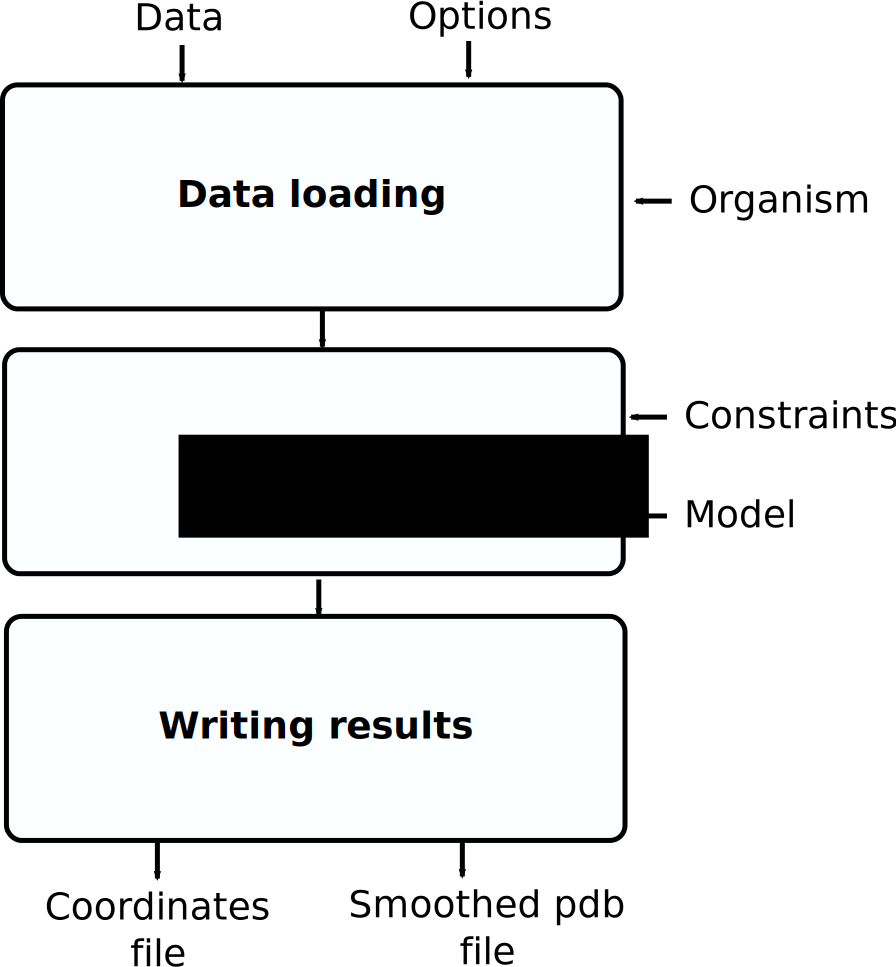
\includegraphics[width=0.6\linewidth]{schema/pastis_old.png}
\end{figure}
\end{frame}

\begin{frame}
\frametitle{More details on the implementation}

{\bf \color{Blue} Data loading}
\begin{itemize}[label={$\bullet$}]
\item Format of the data:
\begin{scriptsize}
\lstinputlisting{scripts/data_format}
\end{scriptsize}
\item The code dealt with changing resolution.
\item Hard coded conversion from counts to wish-distances.
\item Hard coded organism information and constraints.
\end{itemize}
\end{frame}

\begin{frame}
\frametitle{More details on the implementation}
{\bf \color{Blue} Optimization}
\begin{itemize}[label={$\bullet$}]
\item One model (the MDS), implemented in C++
\item Gradients computed and implemented by hand
\item IPOpt for fast high dimensional optimization (newton-type method)
\end{itemize}

\vspace{3em}
\begin{center}
\centering
\includegraphics[width=0.1\linewidth]{images/cpp.png}
\hspace{3em}
\includegraphics[width=0.1\linewidth]{images/coin_banner.png}
\end{center}
\end{frame}

\begin{frame}
\frametitle{More details on the implementation}


{\bf \color{Blue} Writing results}
\begin{itemize}[label={$\bullet$}]
\item Coordinates file structures $(x_1, y_1, z_1, x_2, y_2, z_2, \dots)$
\item Smoothed interpolated structure saved in PDB format file (sometimes not structured properly)
\end{itemize}
\end{frame}

\begin{frame}
\frametitle{My wish: Flexibility and Interactivity}
\begin{itemize}
\item {\bf \color{Blue} Interactivity} 
\begin{itemize}[label={$\bullet$}]
\item being able to launch the code from IPython and interact
with the results
\end{itemize}
\item {\bf \color{Blue} Flexibility}
\begin{itemize}[label={$\bullet$}]
\item Flexible several counts-to-wish-distance mapping.
\item Flexible organism.
\item Flexible constraints.
\item Flexible models.
\end{itemize}
\end{itemize}

\vspace{1em}
{\bf \color{Blue} Fast iteration between code \& results} $\rightarrow$
willing to sacrifice speed for flexibility and fast implementation.
\end{frame}

\begin{frame}
\frametitle{Slowly moving from pure C++ to pure Python}

\begin{itemize}
\item {\bf \color{Blue} Step 1} Creating a Python wrapper using subprocess.
\item {\bf \color{Blue} Step 2} Interfacing the python code with Cython.
\item {\bf \color{Blue} Step 3} Removing all C code.
\end{itemize}
\end{frame}

\begin{frame}
\frametitle{Creating a Python wrapper using subprocess}
\begin{itemize}
\item {\color{Blue} \bf Changing the loading of the data}
\begin{itemize}[label={$\bullet$}]
\item Load the wish-distances instead of the contact counts.
\item Assume the wish-distance matrix is provided at the correct resolution.
\item {\bf \color{Red} No processing done in C++ anymore}
\end{itemize}
\item {\color{Blue} \bf Creating a python package wrapper}
\begin{itemize}[label={$\bullet$}]
\item Python used for all the preprocessing:
\begin{itemize}[label={$\bullet$}]
\item Creating the matrix at the correct resolution (including validation of
the shape of the matrix)
\item Normalizing the data
\end{itemize}
\item And then simply calling the C++ compiled program onto the matrix data.
\end{itemize}
\end{itemize}
\end{frame}

% FIXME add an updated schema

\begin{frame}
\frametitle{Substantial speed up from the data loading}
\begin{itemize}[label={$\bullet$}]
\item The data loading in C++ used to take 45 minutes for a small organism
(\textit{S. cerevisiae})
\item It then took less than 5 minutes.
\end{itemize}

\vspace{3em}
{\color{Red} \bf While C++ is generally faster than Python, it is easy to fall
into unefficient memory management.}

\end{frame}

\begin{frame}
\frametitle{Step 2: using cython for better interfacing}

{\bf \color{Blue} Moving from a hack to a true python wrapper}

\vspace{4em}
\begin{center}
\includegraphics[width=0.3\linewidth]{images/cython.png}
\end{center}
\end{frame}

\begin{frame}
\frametitle{Step 3: switching the optimization to ``Python''}

{\bf \color{Blue} Motivation}: IPOpt relies on hard to install, none opensource
fortran libraries. 
\vspace{2em}
\\
{\bf \color{Blue} Goal}: move to standard python tools to do the optimization.
\vspace{2em}
\\
{\bf \color{Blue} Solution}: use Scipy's optimization toolbox 
\end{frame}

\begin{frame}
\frametitle{Scipy's optimization toolbox}

{\bf\color{Blue} Advantages} \\
\begin{itemize}[label={$\bullet$}]
\item Many optimization algorithms
\item The same interface for all of the optimization algorithms.
\end{itemize}

{
\lstinputlisting[language=Python]{scripts/optimize.py}
}
\end{frame}

\begin{frame}
\frametitle{Step 3: switching the optimization to Python}
{\bf\color{Blue} Implication}
\begin{itemize}[label={$\bullet$}]
\item Reimplement the objective function.
$$
f(x, \delta) = \underset{ij}{\sum}\frac{1}{\delta_{ij}^2} (\|x_i - x_j\| - \delta_{ij})^2
$$
\item Reimplement the gradient.
$$
g(x, \delta) = \frac{\partial f}{\partial x_i}
$$
\item Add the constraints
\end{itemize}
\end{frame}

\begin{frame}
\frametitle{Step 3: switching the optimization to Python}

{
\lstinputlisting[language=Python]{scripts/mds.py}
}

\end{frame}

\begin{frame}
\frametitle{Step 3: switching the optimization to Python}

\begin{itemize}[label={$\bullet$}]
\item Using the L-BFGS-B implementation in Python.
\item No loss of speed.
\item More stable and better convergence.
\item Can easily adapt or remove the constraints for each organism of interest.
\item Can easily change optimization algorithm.
\end{itemize}
\end{frame}

\begin{frame}
\frametitle{An example of 3D structures inferred using \texttt{Pastis}}
\includegraphics[width=\linewidth]{images/3D_var_genes.png}
\end{frame}

\begin{frame}
\frametitle{Conclusion}
\begin{itemize}[label={$\bullet$}]
\item Always use a programming language you are familiar with.
\item If you are not familiar with any programming language, use an ``easy''
programming language (R, Python, etc).
\item In doubt, benchmark to understand where the code is slow.
\item Better algorithms sometimes beat smart implementations.
\end{itemize}
\end{frame}

\begin{frame}
\frametitle{Acknowledgments}
\fboxsep=0pt
\noindent
\begin{minipage}[t]{0.48\linewidth}
\textbf{Mines ParisTech - CBIO} \\
Jean-Philippe \textsc{Vert} \\
Thomas \textsc{Walter} \\

\textbf{UW - Noble lab} \\
William S. \textsc{Noble} \\
Ferhat \textsc{Ay} \\

\textbf{Institut Curie - U900} \\
Emmanuel \textsc{Barillot} \\
Nicolas \textsc{Servant} \\
Chong-Jian \textsc{Chen} \\
Eric \textsc{Viara} \\

\textbf{UMass} \\
Job \textsc{Dekker} \\
Bryan \textsc{Lajoie} \\

\end{minipage}
\hfill%
\begin{minipage}[t]{0.48\linewidth}

\textbf{UC Riverside} \\
Karine \textsc{Le Roch} \\
Sebastiaan \textsc{Bol} \\
Evelien \textsc{Bunnik} \\
Jacques \textsc{Prudhomme} \\

\textbf{Institut Curie - UMR168} \\
Edith \textsc{Heard} \\

\textbf{UW - Dunham lab} \\
Maitreya \textsc{Dunham} \\
Ivan \textsc{Liachko} \\

\textbf{UW - Shendure lab} \\
Jay \textsc{Shendure} \\
Josh \textsc{Burton} \\

\end{minipage}

\end{frame}

\begin{frame}[allowframebreaks,noframenumbering]
  \frametitle{References}
  \bibliographystyle{plainnat}
  \bibliography{refs}
\end{frame}

\end{document}

